%3.1.tex
LLVMは2000年にイリノイ大学で開発が開始されたコンパイラ基盤である.コンパイラ基盤とはコンパイラに必要となるモジュールをまとめたもので,コンパイラを開発するためのフレームワークである.
LLVMの構成を図\ref{fig:LLVM}に示す.LLVMはソースコードをLLVMの中間表現であるLLVM IRに変換するフロントエンド,LLVM IRに対して最適化等の操作やLLVM IRから機械語やアセンブリコードへの変換を行うバックエンドに分かれている.中間表現であるLLVM IRは階層構造のドメイン固有言語である.
LLVMではこれらの機能がモジュール化されており,独自機能を実装する以外は既存のものを再利用することができる.例えば新たなアーキテクチャ向けのコンパイラを開発する際はバックエンドのみ実装を行い,フロントエンドについては再利用することができる.

\begin{figure}[tb]
    \centering
    \includegraphics[scale=0.4]{image/LLVM.pdf}
    \caption{LLVMの構成}
    \label{fig:LLVM}
\end{figure}

LLVMには既にRISC-Vを対象としたコード生成のためのバックエンドが実装されている.本研究ではRISC-Vを独自にベクトル拡張したベクトル拡張付きRISC-Vの命令の生成を目的としているため,このRISC-V向けのバックエンドに対して変更を加えることによって独自命令の生成を行う.

LLVMバックエンドにおけるコード生成の流れを図\ref{fig:LLVM_backend}に示す.
LLVMバックエンドではPassによって処理が行われる.図\ref{fig:LLVM_backend}
ではLLVMバックエンドにおけるデータフォーマットの変化と実行されるPassを表している.

\begin{figure}[tb]
    \centering
    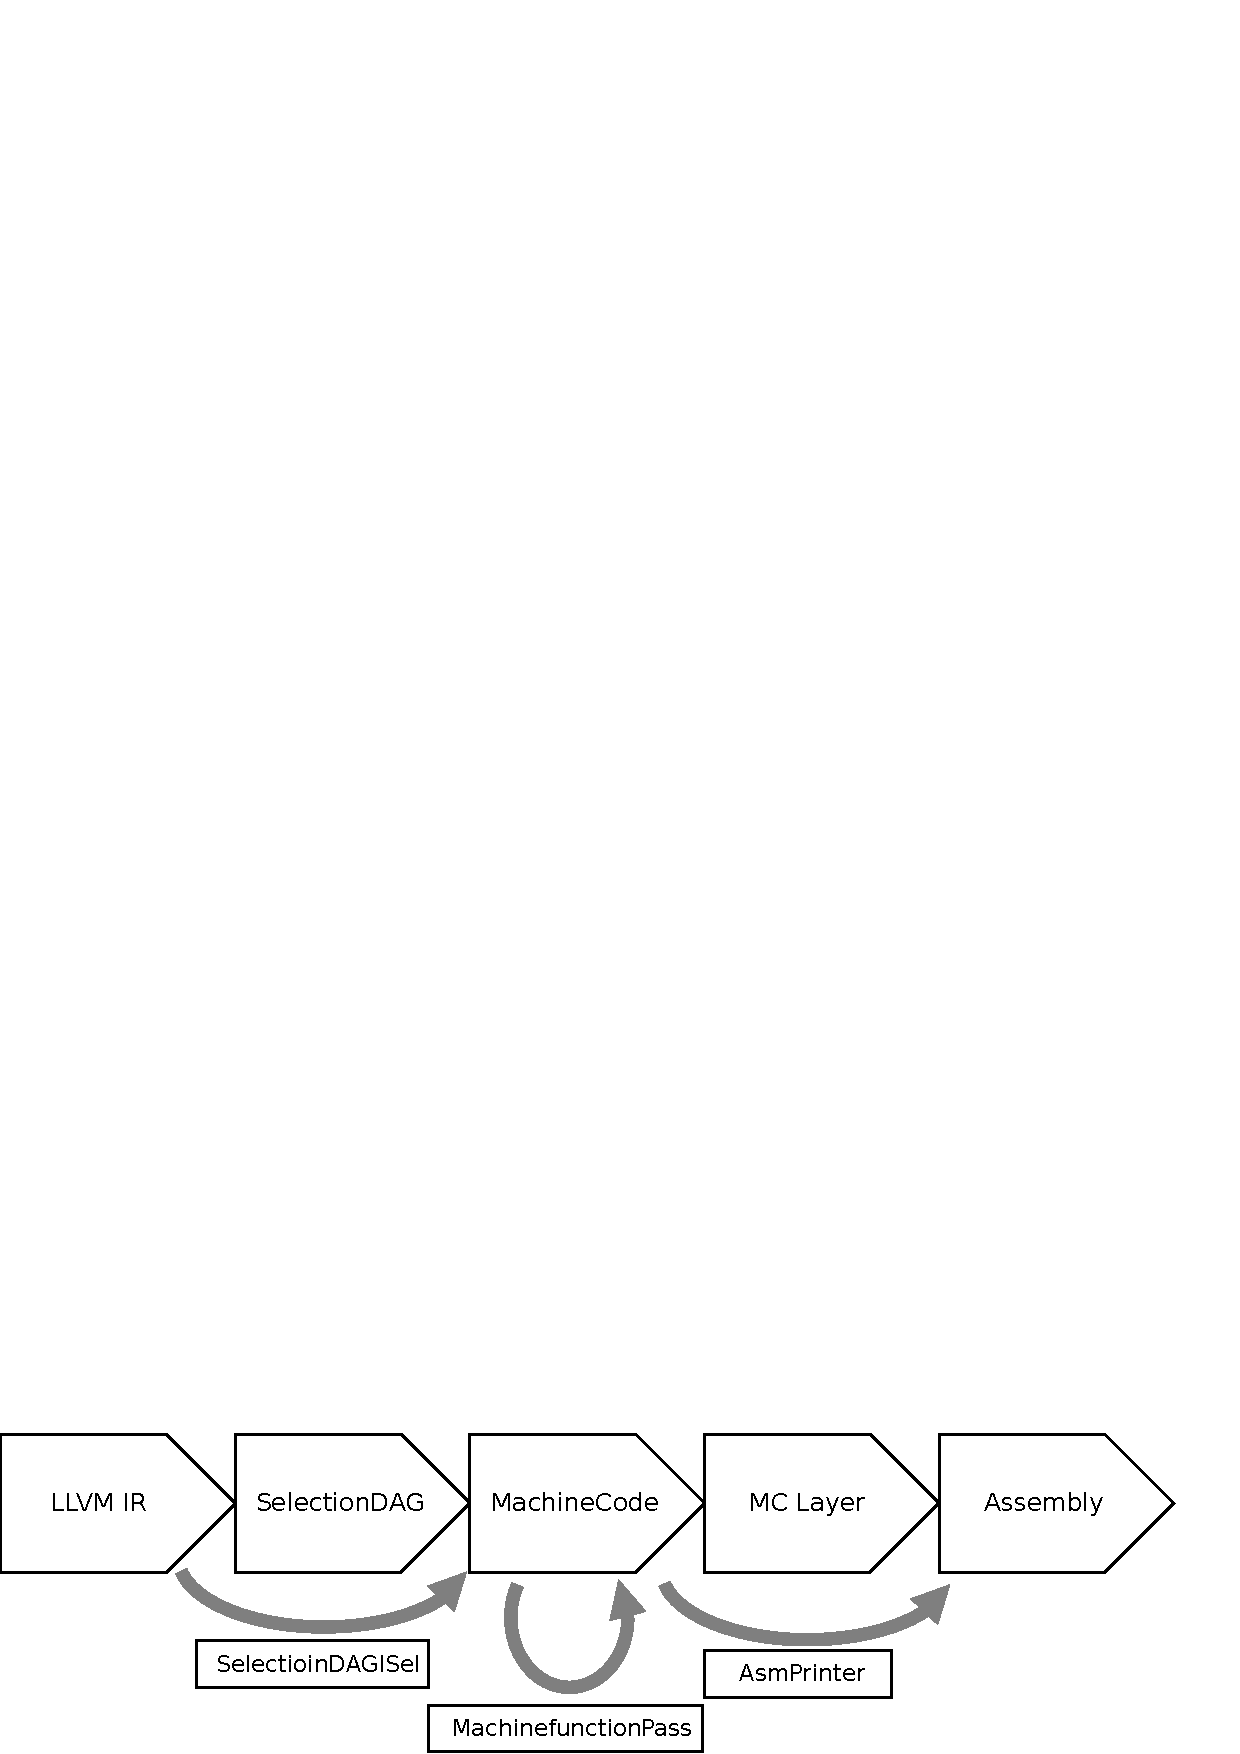
\includegraphics[scale=0.7]{image/backend.pdf}
    \caption{LLVMバックエンド}
    \label{fig:LLVM_backend}
\end{figure}

バックエンドではLLVM IRからDAG (Directed Acyclic Graph)であるSelectionDAGへフォーマットを変換する.SelectionDAGはLLVM IRをグラフ形式で表したもので,各命令やデータの依存関係を表現する.SelectionDAGへの変換はSelectionDAGISelパスで行われ,SelectionDAGは最終的にSelectionDAGISelパスによってMachineCod形式に変換される.SelectionDAGISelではLower,Combine,Legalize,Select,Scheduleのフェーズから構成される.

LowerはLLVM IRからSelectionDAGに変化させるフェーズである.このフェーズではLLVM IRからSelectionDAGのノードへと一対一の対応を行う.この段階ではターゲットマシンでは利用できない命令やデータ形式を含んでる不正 (illegal)な状態である.

Combineフェーズではパターンマッチングによる置き換えで最適化を行い,命令の単純化を行う.

Legalizeはターゲットマシンではサポートされていない命令やデータ形式を他のものに置き換えるフェーズである.このフェーズによって不正な状態であったSelectionDAGノードが正当 (legal)な状態となる.

SelectフェーズではSelectionDAGのノードをターゲットマシンの命令を含んだMachineNodeへと変換する.

Scheduleフェーズでは構築されたグラフの依存関係を元に命令をスケジューリングするフェーズである.

SelectionDAGISelパスではこれらのすべてのフェーズが終わった後にMachineCodeを出力する.

MachinefunctionパスではMachineCodeという形式を扱う.この形式はLLVM IRと似た構成になっているが,より機械語に近い表現になっている.
MachineCodeがSelectionDAGISelによって生成された直後はまだ命令で扱うレジスタは無限個あると仮定した仮想レジスタやphi関数を含んだSSA (Static Single Assignment form)形式で表現されている.MachinefunctionPassではレジスタの割当やphi命令の削除を行い,MachineCodeを非SSA形式へと変換する.

AsmPrinterパスはMachineCodeをMC Layer形式へと変換した後にアセンブリコードなどを出力するパスである.MC Layer形式はMachineCode形式のような階層構造がない形式であり,アセンブリコードへの変換だけでなく,オブジェクトファイルへの変換のための形式である.

